\section{The Graphical User Interface}
\label{sec:gui}

The graphical user interface (GUI) of QKD-Simulate is shown in Figure \ref{fig:gui}. It is based on the Qt library and is mainly constructed in the \texttt{main\_widget} class (defined in \texttt{main\_widget.h} and \texttt{main\_widget.cpp}) by the \texttt{setup\_widget()} function. This class also contains a channel object (defined as member \texttt{channel * m\_cChannel}) that simulates the quantum channel as described in the previous sections.

The elements of the GUI will be described in the following subsections. When changing parameter values inside the parameter text boxes, attention should always be paid especially to the status bar at the bottom of the GUI main window, because in the case that some parameters cannot be set due to an out-of-range error, an error message is displayed in the status bar.

\begin{figure}[p]
\centering
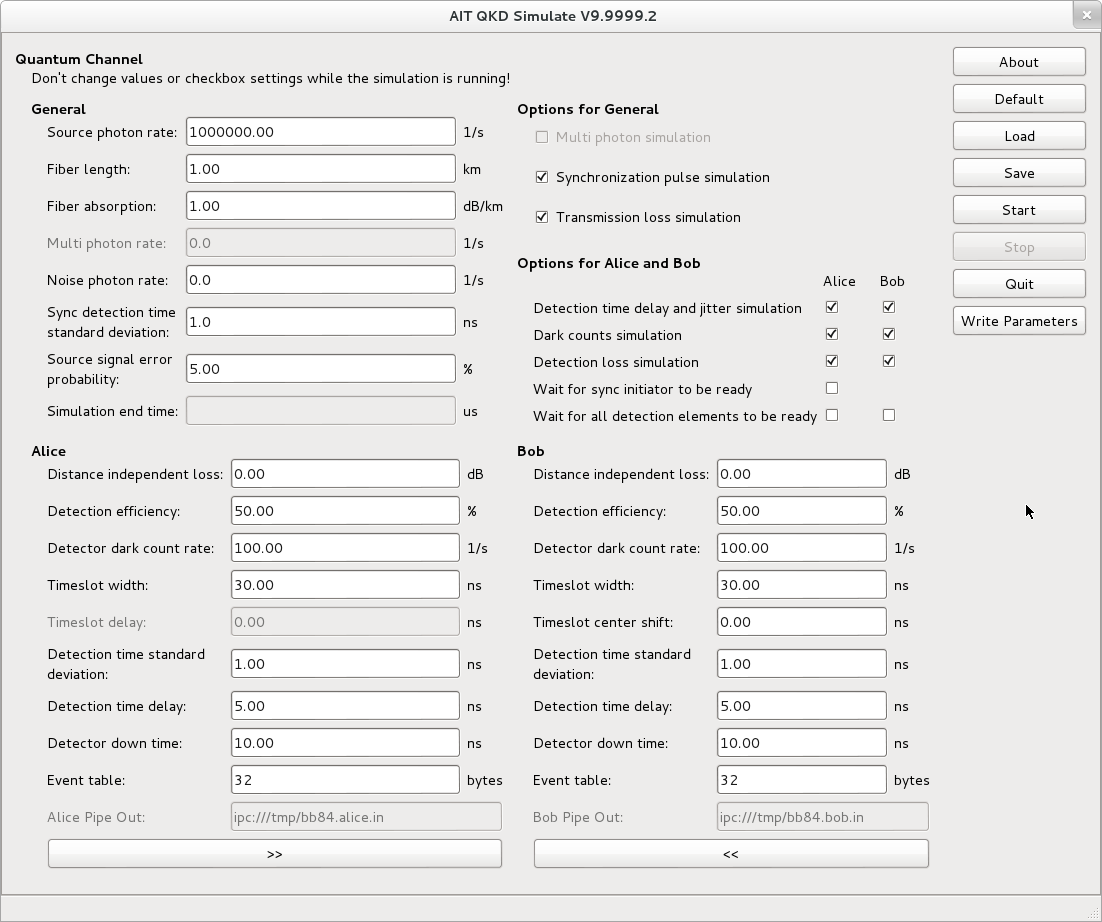
\includegraphics[angle=90,width=\textwidth,keepaspectratio]{images/gui.png}
\caption{The graphical user interface}
\label{fig:gui}
\end{figure}

\refstepcounter{footnote}
\newcounter{fnmodinfo}
\setcounter{fnmodinfo}{\value{footnote}}

\subsection{General Inputs}
\label{subsec:gui_general}

\subsubsection{Source photon rate}
The rate at which photon pairs are generated by \textbf{source}. Photon pair generation is assumed to be a Poisson process so that the time between each pair of consecutive photon generation events has an exponential distribution.

Modifying this input parameter effects a change of the following properties\hyperlink{fn:modinfo}{\footnotemark[\value{fnmodinfo}]}:\\
\texttt{m\_cChannel->m\_cSource.m\_nPhotonRate}

\footnotetext[\value{fnmodinfo}]{\hypertarget{fn:modinfo}A change of the listed properties may also cause further changes of other properties in consequence - refer to the descriptions of the specific components in section \ref{sec:comp} for further information.}

\subsubsection{Fiber length}
The length of the quantum transmission fiber and the sync pulse transmission fiber. Note that the length parameter is only used to simulate transmission loss according to the specified fiber absorption (see subsection \ref{subsubsec:gui_general_fiber_absorption}) in case that the ``Transmission loss simulation'' checkbox has been checked (see subsection \ref{subsubsec:gui_general_options_transmission_loss_simulation}), but no fiber delay is simulated, because ignoring it does not essentially change the simulation behaviour (except for a time shift) but helps to speed up the simulation and to reduce the simulators memory usage.

Modifying this input parameter effects a change of the following properties\hyperlink{fn:modinfo}{\footnotemark[\value{fnmodinfo}]}:\\
\texttt{m\_cChannel->m\_cFiber.m\_nLength}

\subsubsection{Fiber absorption}
\label{subsubsec:gui_general_fiber_absorption}
The quantum transmission fiber's absorption coefficient. Note that the sync pulse transmission fiber is assumed to be lossless.

Modifying this input parameter effects a change of the following properties\hyperlink{fn:modinfo}{\footnotemark[\value{fnmodinfo}]}:\\
\texttt{m\_cChannel->m\_cFiber.m\_nAbsorptionCoefficient}

\subsubsection{Noise photon rate}
The rate of noise photons generated by the \textbf{noise photon source} located inside \textbf{fiber}. It is assumed that noise photon generation is a Poisson process and that the generated noise photons are non-polarised.

Modifying this input parameter effects a change of the following properties\hyperlink{fn:modinfo}{\footnotemark[\value{fnmodinfo}]}:\\
\texttt{m\_cChannel->m\_cFiber.m\_noise\_photon\_source.m\_noise\_photon\_rate}

\subsubsection{Sync detection time standard deviation}
The jitter assigned to the \textbf{sync pulse receiver} for sync pulse detection. A Gaussian distribution of the jitter is assumed, except for a cutoff at minus five standard deviations (refer to sections \ref{subsec:comp_channel} and \ref{par:comp_detector_syncprcv} for further information on the influence of this parameter).

Modifying this input parameter effects a change of the following properties\hyperlink{fn:modinfo}{\footnotemark[\value{fnmodinfo}]}:\\
\texttt{m\_cChannel->m\_nStndSyncDeviation}

\subsubsection{Source signal error probability}
Whenever the \textbf{source} generates an entangled photon pair, the \texttt{entanglement\_error} property of the generated \texttt{photon\_pair} object (see section \ref{subsec:concepts_photons}) is set according to the value specified for the source signal error probability.

Modifying this input parameter effects a change of the following properties\hyperlink{fn:modinfo}{\footnotemark[\value{fnmodinfo}]}:\\
\texttt{m\_cChannel->m\_cSource.m\_nSignalErrorProbablity}

\subsubsection{Simulation end time}
The time until which the simulation (starting from time 0) should run. This value is only used in \textit{free running mode}.

Modifying this input parameter effects a change of the following properties\hyperlink{fn:modinfo}{\footnotemark[\value{fnmodinfo}]}:\\
\texttt{m\_cChannel->m\_ch\_event\_manager.m\_sim\_end\_time}

\subsection{General Options}
\label{subsec:gui_general_options}

\subsubsection{Synchronization pulse simulation}
\label{subsubsec:gui_general_syncpulse}
If this checkbox is checked, the \textit{sync mode} or one of its variants (depending on the settings described in subsections \ref{subsubsec:gui_abopt_wait_for_sync_initiator} and \ref{subsubsec:gui_abopt_wait_for_all}) is used. If it is not checked, \textbf{detector alice} and \textbf{detector bob} are set in \textit{free running mode}.

Changing this option effects a change of the following properties\hyperlink{fn:modinfo}{\footnotemark[\value{fnmodinfo}]}:\\
\texttt{m\_cChannel->m\_cDetectorAlice->m\_detection\_mode}\\
\texttt{m\_cChannel->m\_cDetectorBob->m\_detection\_mode}

\subsubsection{Transmission loss simulation}
\label{subsubsec:gui_general_options_transmission_loss_simulation}
If this checkbox is checked, the fiber absorption coefficient as described in subsection \ref{subsubsec:gui_general_fiber_absorption} is assigned to the quantum transmission fiber. If it is not checked, the quantum transmission fiber is simulated to be lossless.

Changing this option effects a change of the following properties\hyperlink{fn:modinfo}{\footnotemark[\value{fnmodinfo}]}:\\
\texttt{m\_cChannel->m\_cFiber.m\_bLoss}

\subsection{Alice Inputs}
\label{subsec:gui_alice}

\subsubsection{Distance independent loss}
A distance independent loss assigned to the \textbf{detector optics} of \textbf{detector alice}.

Modifying this input parameter effects a change of the following properties\hyperlink{fn:modinfo}{\footnotemark[\value{fnmodinfo}]}:\\
\texttt{m\_cChannel->m\_cDetectorAlice.m\_nLossRate}

\subsubsection{Detection efficiency}
A detection efficiency assigned to the \textbf{detector optics} of \textbf{detector alice}.

Modifying this input parameter effects a change of the following properties\hyperlink{fn:modinfo}{\footnotemark[\value{fnmodinfo}]}:\\
\texttt{m\_cChannel->m\_cDetectorAlice.m\_nEfficiency}

\subsubsection{Detector dark count rate}
The dark count rate for \textbf{detector alice}. This detector dark count rate is assigned as dark count rate parameter to each of the four \textbf{detection element}s. Dark counts for all detection elements are assumed to be Poisson processes, but they can only occur if the specific detection element is enabled and ready (not in down state).

Modifying this input parameter effects a change of the following properties\hyperlink{fn:modinfo}{\footnotemark[\value{fnmodinfo}]}:\\
\texttt{m\_cChannel->m\_cDetectorAlice.m\_nDarkCountRate}

\subsubsection{Timeslot width}
The duration of the window produced by the \textbf{window generator}.

Modifying this input parameter effects a change of the following properties\hyperlink{fn:modinfo}{\footnotemark[\value{fnmodinfo}]}:\\
\texttt{m\_cChannel->m\_cDetectorAlice.m\_nTimeSlotWidth}

\subsubsection{Detection time standard deviation}
\label{subsubsec:gui_alice_det_time_stnd_dev}
The jitter of photon detection set for the four \textbf{detection element}s. A Gaussian distribution of jitter is assumed.

Modifying this input parameter effects a change of the following properties\hyperlink{fn:modinfo}{\footnotemark[\value{fnmodinfo}]}:\\
\texttt{m\_cChannel->m\_cDetectorAlice.m\_nPhotonTimeStndDeviation}

\subsubsection{Detection time delay}
\label{subsubsec:gui_alice_det_time_delay}
The delay of photon detection set for the four \textbf{detection element}s. Note that this parameter should always be set to a value greater or equal than at least three times the detection time standard deviation (see subsection \ref{subsubsec:gui_alice_det_time_stnd_dev}), because acausal detection times are not allowed in the simulation and if they would occur, the random variable for the jitter time is ``reshuffled'' until a causal detection time (sum of delay time plus jitter time) is obtained. This effectively causes the originally Gaussian probability distribution of detection times to be cut off at zero and therefore a distortion to a non-Gaussian distribution. This effect rarely occurs, however, if the detection time delay is set to at least three times the detection time standard deviation, as recommended.

Modifying this input parameter effects a change of the following properties\hyperlink{fn:modinfo}{\footnotemark[\value{fnmodinfo}]}:\\
\texttt{m\_cChannel->m\_cDetectorAlice.m\_nPhotonTimeDelay}

\subsubsection{Detector down time}
The down time configured for the \textbf{detection element}s.

Modifying this input parameter effects a change of the following properties\hyperlink{fn:modinfo}{\footnotemark[\value{fnmodinfo}]}:\\
\texttt{m\_cChannel->m\_cDetectorAlice.m\_nDownTime}

\subsubsection{Event table}
The size of the \textbf{event buffer}'s key buffer in bytes. Each byte can store the contents of the event latch for two sync pulses (for the first sync pulse, the upper half byte is filled, and for the second sync pulse the lower half byte is filled). The bit ordering used for the four detection elements is (from high to low bit): M P V H (minus, plus, vertical, horizontal). 

Modifying this input parameter effects a change of the following properties\hyperlink{fn:modinfo}{\footnotemark[\value{fnmodinfo}]}:\\
\texttt{m\_cChannel->m\_cDetectorAlice.m\_nEventTableSize}

\subsection{Bob Inputs}

The inputs for Bob are almost the same as for Alice, therefore only the differences to Alice's side are explained.

\subsubsection{Timeslot center shift}
This parameter specifies the mean time shift between the center of the window generated by Bob's \textbf{window generator} and the associated photon coming to \textbf{detector bob}. A positive value specifies that the photon comes later than the center of the window, a negative value specifies that the photon comes earlier.

Modifying this input parameter effects a change of the following properties\hyperlink{fn:modinfo}{\footnotemark[\value{fnmodinfo}]}:\\
\texttt{m\_cChannel->m\_timeslot\_center\_shift}

\subsection{Options for Alice and Bob}
\label{subsec:gui_abopt}

\subsubsection{Detection time delay and jitter simulation}
If this checkbox is checked, delay and jitter times are simulated for the \textbf{detection element}s. If it is unchecked, the delay and jitter times for the \textbf{detection element}s are set to zero.

Changing these options effects a change of the following properties (for Alice or Bob, respectively)\hyperlink{fn:modinfo}{\footnotemark[\value{fnmodinfo}]}:\\
\texttt{m\_cChannel->m\_cDetectorAlice->m\_bJitter}\\
\texttt{m\_cChannel->m\_cDetectorBob->m\_bJitter}

\subsubsection{Dark counts simulation}
If this checkbox is checked, dark counts are simulated for the \textbf{detection element}s. If it is unchecked, the dark count rate of the \textbf{detection element}s is set to zero.

Changing these options effects a change of the following properties (for Alice or Bob, respectively)\hyperlink{fn:modinfo}{\footnotemark[\value{fnmodinfo}]}:\\
\texttt{m\_cChannel->m\_cDetectorAlice->m\_bDarkCounts}\\
\texttt{m\_cChannel->m\_cDetectorBob->m\_bDarkCounts}

\subsubsection{Detection loss simulation}
If this checkbox is checked, the distance independent loss, detection efficiency and detector down time parameters are assigned to the specific detector. If this checkbox is not checked, the detector is simulated to be lossless and to have zero down time.

Changing these options effects a change of the following properties (for Alice or Bob, respectively)\hyperlink{fn:modinfo}{\footnotemark[\value{fnmodinfo}]}:\\
\texttt{m\_cChannel->m\_cDetectorAlice->m\_bLoss}\\
\texttt{m\_cChannel->m\_cDetectorBob->m\_bLoss}

\subsubsection{Wait for sync initiator to be ready}
\label{subsubsec:gui_abopt_wait_for_sync_initiator}
If this checkbox is checked and the ``Wait for all detectors to be ready'' for Alice is not checked, \textbf{detector alice} is set into \textit{sync mode - wait for sync initiator to be ready}. If this checkbox is not checked (or not available (for Bob's side), respectively) and the ``Wait for all detectors to be ready'' checkbox is also unchecked but the ``Synchronization pulse simulation'' checkbox is checked (see section \ref{subsubsec:gui_general_syncpulse}), the specific \textbf{detector} is set into \textit{sync mode}.

Changing this option effects a change of the following properties\hyperlink{fn:modinfo}{\footnotemark[\value{fnmodinfo}]}:\\
\texttt{m\_cChannel->m\_cDetectorAlice->detection\_mode}

\subsubsection{Wait for all detection elements to be ready}
\label{subsubsec:gui_abopt_wait_for_all}
If this checkbox is checked, the specific detector is set into \textit{sync mode - wait for all detection elements to be ready}. If this checkbox is not checked and the ``Wait for sync initiator to be ready'' checkbox is also not checked (or not available (for Bob's side), respectively) but the ``Synchronization pulse simulation'' checkbox is checked (see section \ref{subsubsec:gui_general_syncpulse}), the specific \textbf{detector} is set into \textit{sync mode}.

Changing these options effects a change of the following properties (for Alice or Bob, respectively)\hyperlink{fn:modinfo}{\footnotemark[\value{fnmodinfo}]}:\\
\texttt{m\_cChannel->m\_cDetectorAlice->detection\_mode}\\
\texttt{m\_cChannel->m\_cDetectorBob->detection\_mode}

\subsection{Click Buttons}

\subsubsection{About}
Displays the ``About'' dialog box.

\subsubsection{Default}
Loads the default values for the parameters, which are defined in \texttt{default\_values.cpp}.

\subsubsection{Load}
Opens a dialog box that allows to select a configuration file from which parameters should be loaded.

\subsubsection{Save}
Open a dialog box that allows to save the configured parameters to a configuration file. Note that checkbox settings are not stored in the configuration file.

\subsubsection{Start}
Start the quantum channel simulation.

\subsubsection{Stop}
Terminate the quantum channel simulation.

\subsubsection{Quit}
Terminate the QKD-Simulate program.